\begin{center}
\begin{minipage}{0.49\textwidth}
\begin{center}
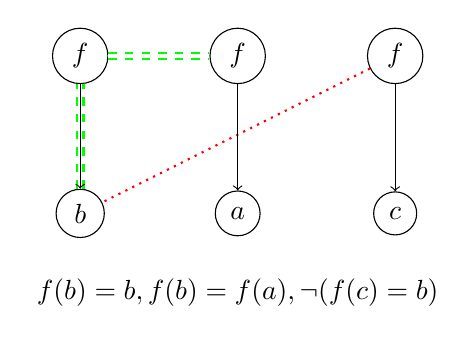
\begin{tikzpicture}
\node (b) [draw, circle, minimum size=0.8, align=center] at (0,0) {$b$};
\node (a) [draw, circle, minimum size=0.8, align=center] at (2,0) {$a$};
\node (c) [draw, circle, minimum size=0.8, align=center] at (4,0) {$c$};
\node (f1) [draw, circle, minimum size=0.8, align=center] at (0,2) {$f$};
\node (f2) [draw, circle, minimum size=0.8, align=center] at (2,2) {$f$};
\node (f3) [draw, circle, minimum size=0.8, align=center] at (4,2) {$f$};

\draw [double, dashed, thick, green, double distance=1.5] (b) -- (f1);
\draw [double, dashed, thick, green, double distance=1.5] (f1) -- (f2);
\draw [red, dotted, thick] (f3) -- (b);
\draw [->] (f1) -- (b);
\draw [->] (f2) -- (a);
\draw [->] (f3) -- (c);

\node [align=center] at (2, -1) {$f(b) = b, f(b)=f(a), \lnot(f(c)=b)$};
\end{tikzpicture}
\end{center}
\end{minipage}
\begin{minipage}{0.49\textwidth}
\begin{center}
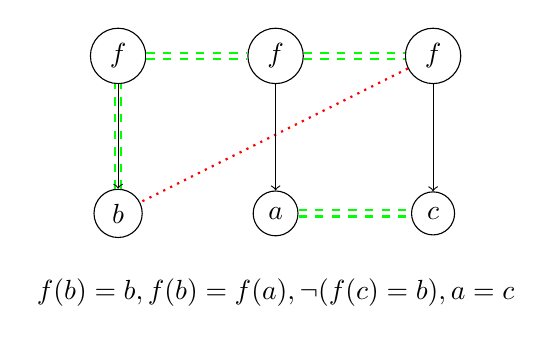
\begin{tikzpicture}
\node (b) [draw, circle, minimum size=0.8, align=center] at (0,0) {$b$};
\node (a) [draw, circle, minimum size=0.8, align=center] at (2,0) {$a$};
\node (c) [draw, circle, minimum size=0.8, align=center] at (4,0) {$c$};
\node (f1) [draw, circle, minimum size=0.8, align=center] at (0,2) {$f$};
\node (f2) [draw, circle, minimum size=0.8, align=center] at (2,2) {$f$};
\node (f3) [draw, circle, minimum size=0.8, align=center] at (4,2) {$f$};

\draw [double, dashed, thick, green, double distance=1.5] (b) -- (f1);
\draw [double, dashed, thick, green, double distance=1.5] (f1) -- (f2);
\draw [double, dashed, thick, green, double distance=1.5] (a) -- (c);
\draw [double, dashed, thick, green, double distance=1.5] (f2) -- (f3);
\draw [red, dotted, thick] (f3) -- (b);
\draw [->] (f1) -- (b);
\draw [->] (f2) -- (a);
\draw [->] (f3) -- (c);

\node [align=center] at (2, -1) {$f(b) = b, f(b)=f(a), \lnot(f(c)=b), a=c$};
\end{tikzpicture}
\end{center}
\end{minipage}
\captionof{figure}{Example E-graphs}
\end{center}
